
\documentclass{proposal}
\usepackage{verbatim}
\usepackage{graphicx}
\usepackage{amsmath,amssymb}
\graphicspath{ {./plot/} }
\usepackage{svg}

\degree{Doctor of Philosophy}
\department{Electrical Engineering}
\gradyear{2019}
\author{Jiexin (Alice) Gao}
\title{Predicting in vivo RNA Secondary Structure}

\setcounter{tocdepth}{2}

\flushbottom

\begin{document}

\begin{preliminary}

\maketitle

%\begin{abstract}
%
%
%
%\end{abstract}

\tableofcontents

\end{preliminary}





\chapter{Introduction}




Once believed to be an intermediate molecule that serves as messenger between DNA and protein,
RNA is now known to be involved in many aspects in gene regulation and expression.
Unlike DNA which forms stable double helix, RNA predominantly stays single-stranded and folds onto itself by
forming base pairs via hydrogen bonds, including Watson-Crick pair A-U, G-C and non-canonical pair A-U.
Nearby paired and unpaired bases further assemble into
hairpins, bulges, internal loops, Multi loops and pseudoknots.
In addition, secondary structures within an RNA molecule can interact via non-covalent bond, to form tertiary structure.


RNA secondary and tertiary structure play key roles in regulating both coding and nocoding genes,
affecting all steps including transcription, splicing, polyadenylation, translation,
localization and stability\cite{wan2011understanding, mortimer2014insights, bevilacqua2016genome}.
Over the past few years, combination of RNA structure probing and high throughput sequencing has enabled
the measurement of genome-wide RNA structural at single nucleotide resolution in multiple organisms and cell types,
which provides new insight into the relationship between RNA structure and its function.

\section{High throughput probing of RNS secondary structure}

Two types of reagents are being used to probe RNA structures: enzymes and chemicals.
These reagents cleave or modify RNA at specific bases and/or structured regions.

Parallel analysis of RNA structures (PARS)\cite{wan2014landscape}
uses RNase S1 to cleave single-stranded regions, and RNase V1 to cleave double-stranded regions.
Similarly, fragmentation sequencing (FragSeq)\cite{underwood2010fragseq} utilizes RNase P1 to cleave single-stranded RNA.
After high throughput sequencing and read alignment to the genome or transcriptome,
the locations of cleavage can be determined.
In PARS, the ratio between V1 and S1 is calculated (PARS score),
and in FragSeq, the ratio between RNase P1 treated and untreated control is calculated.


Dimethyl sulfide (DMS) reacts with unpaired adenine (A) and cytosine (C),
and is being used in various protocols to modify RNA\cite{rouskin2014genome, talkish2014mod}.
selective 2-hydroxyl acylation analysed by primer extension (SHAPE)
method uses the chemical N-methylisotoic anhydride (NMIA) and its derivatives to
modifiy the ribose of nucleotides within flexible regions in RNA secondary structure,
and is able to react with all four nucleotides.
In both cases, the modified nucleotides result in termination of reverse transcription (RT),
and can be detected via high throughput sequencing.
The number of RT stops at each position is thus indicative of the relative accessibility of that nucleotide.

In addition to measuring the accessibility of a single nucleotide,
effort is underway to probe the actual base-pairing, either intramolecular, or intermolecular.
Three methods have been proposed to use psoralens for cross-linking the duplex regions of RNA:
psoralen analysis of RNA interactions and structures (PARIS)\cite{lu2018paris},
sequencing of psoralen crosslinked, ligated, and selected hybrids (SPLASH)\cite{aw2016vivo}, and
ligation of interacting RNA and high-throughput sequencing (LIGR-seq)\cite{sharma2016global},
Sequencing of the fragmented and ends-ligated reads provides information on direct base-pairing in secondary structure and \textit{trans} RNA-RNA interactions.


\begin{figure}[h!]
    \centering
    \includegraphics[width=0.9\textwidth]{probing_methods.png}
    \caption{RNA structure probing methods. From Piao et. al\cite{piao2017rna}.}
    \label{fig:probing_methods}
    \centering
\end{figure}



Different probing methods have their own limitations.
Enzymes are too big to permeate through cell membranes, thus can not be used \textit{in vivo}.
Certain enzymes requires non-physiological condition to be acitve,
for example, RNase V1 needs much higher $Mg^{2+}$, while $Mg^{2+}$ is known to promote RNA folding.
Chemicals such as Dimethyl sulfide (DMS) works \textit{in vivo},
but it only detects unstructured A/C bases.
Cross-link methods were proposed very recently, and more work needs to be done to fully understand
 the bias and error involved in experimental protocol and read processing.
For example, it has been hypothesized that perfectly ordinary duplexes such as those
involving G-C base pairs might not be detectable due to the bias of cross-linking pyrimidines\cite{stefanov2018deciphering}.

Furthermore, although \textit{in vitro} data provides invaluable insight into the genome-wide organization of RNA structure,
it has been demonstrated in various organisms that \textit{in vivo} structure can differ significantly from \textit{in vitro}.
In a living cell environment, the presence of proteins and ligands,
concentration of salt, temperature and other factors defines a complex environment, which in turn affects RNA structure,
and the precise reconstruction of these conditions in vitro is almost impossible.
Rouskin et al.\cite{rouskin2014genome} studied yeast RNA structure and found that RNAs are less structured in vivo than in vitro.
Moreover, they observed that structures unfold when $Mg^{2+}$ is lowered \textit{in vitro},
and more structured regions emerge when cell is depleted of ATP \textit{in vivo}.
%(which underscores the importance of in vivo probing that captures the specific
%physiological condition of the cell type of interest.




\section{RNA secondary structure and gene regulation}

Genome-wide RNA structure probing has enabled the analysis of structure and function at a global scale,
which uncovers new properties and relationship that was never discovered from previous studies.

\subsection*{Transcription}

Kertesz et. al\cite{kertesz2010genome} performed in vitro profiling of the budding yeast
(\textit{Saccharomyces cerevisiae}) RNA structure using PARS.
Averaging PARS scores across more than $3000$ mRNAs revealed a unique pattern across the transcript (Fig \ref{fig:yeast_cds_utr}):
 the UTRs are less structured than the CDS, both start and stop codon are significantly more accessible,
and the coding region exhibits a three nucleotide periodical pattern,
where the first nucleotide is more accessible and the second one is less accessible.

In contrary, although RNAs in human show a similar start/stop codon accessibility and CDS periodicity,
it was observed that UTRs are only slightly less structured than CDS\cite{wan2014landscape}.


\begin{figure}[h!]
    \centering
    \includegraphics[width=0.8\textwidth]{yeast_cds_utr.png}
    \caption{Yeast RNA structure differ in CDS and UTR. From Kertesz et. al\cite{kertesz2010genome}.}
    \label{fig:yeast_cds_utr}
    \centering
\end{figure}



\subsection*{Splicing}

Wan et. al\cite{wan2014landscape} analyzed human lymphoblastoid cell lines from a parent-offspring trio by PARS,
and observed less structure at AG dinucleotide in the upstream exon donor site,
and more structure at the first nucleotide in the downstream acceptor site, as shown in Fig \ref{fig:exon_exon_junction}.
This suggests a potential regulatory role of RNA structure in efficient splicesome assembly.


\begin{figure}[h!]
    \centering
    \includegraphics[width=0.4\textwidth]{exon_exon_junction.png}
    \caption{RNA structure at exon-exon junction in human lymphoblastoid cell lines. From Wan et. al\cite{wan2014landscape}.}
    \label{fig:exon_exon_junction}
    \centering
\end{figure}


\subsection*{Polyadenylation}

Ding et. al\cite{ding2014vivo} used Structure-Seq (TODO review) to study the genome-wide RNA structure of
\textit{Arabidopsis thaliana} seedlings \textit{in vivo} and discovered a pattern around alternative polyadenylation sites across $5959$ mRNAs.
As shown in Fig \ref{fig:poly_a}, region upstream of the site (-15nt to -2nt) is significantly more structured, as indicated by lower reactivity,
and region downstream of the site (-1nt to +5nt) is significantly less structured, as indicated by higher reactivity.
This

\begin{figure}[h!]
    \centering
    \includegraphics[width=0.6\textwidth]{poly_a.png}
    \caption{RNA structure around alternative polyadenylation sites in \textit{Arabidopsis thaliana}. From Ding et. al\cite{ding2014vivo}.}
    \label{fig:poly_a}
    \centering
\end{figure}





\subsection*{Translation}

Kertesz et. al\cite{kertesz2010genome} reported a small but significant anti-correlation between PARS scores 10bp upstream
of the start codon and ribosome density throughout the transcript.
In addition, genes where 5'UTRs are less structured than the beginning of the coding region also show a tendency towards higher ribosome density.

\subsection*{Localization}

Kertesz et. al\cite{kertesz2010genome} discovered increased structure in coding region for genes
whose encoded proteins localize to distinct cellular domains or function in specific metabolic pathways.
On the other hand, ribosomal transcripts show less structure in UTR and CDS (Fig \ref{fig:yeast_localization}).



\begin{figure}[h!]
    \centering
    \includegraphics[width=0.4\textwidth]{yeast_localization.png}
    \caption{RNA structure in CDS and UTR affects localization in yeast. From Kertesz et. al\cite{kertesz2010genome}.}
    \label{fig:yeast_localization}
    \centering
\end{figure}



\subsection*{Stability}


Kertesz et. al\cite{kertesz2010genome} discribed how RNA structure in UTR regulates gene expression during heat shock in order to conserve energy.
Certain class of genes (e.g. ribosomal encoding RPL1A) with less UTR structure becomes unfolded with increased temperature,
which allows degradation by exosome, thus tuning down translation.
On the other hand, genes with more UTR structure like chaperones and unfolded response proteins (e.g. HAC1 and PTC2) remain stable and expressed (Fig \ref{fig:yeast_stability}).

\begin{figure}[h!]
    \centering
    \includegraphics[width=0.6\textwidth]{yeast_stability.png}
    \caption{Yeast gene expression regulation via RNA structure during heat shock. From Mortimer et. al\cite{mortimer2014insights}.}
    \label{fig:yeast_stability}
    \centering
\end{figure}





\section{Deep neural network for sequence modelling}

Predicting RNA structure is similar in its nature to many applications in
computer vision (CV) and natural language processing(NLP),
where the input is a variable sized sequence,
and the output is a sequence of the same size as the input.
Here we review the recent breakthroughs in deep learning related to sequence modelling and discuss their application in genomics.
(TODO 2D MAP)


\subsection*{Recurrent neural network and LSTM}

Recurrent neural networks(RNNs), especially long short-term memory (LSTM)\cite{hochreiter1997long},
have been successfully applied to many sequence labelling tasks
Although LSTM mitigates the vanishing and exploding gradient problem in the vanilla RNNs,
and has the nice property of being able to model long range dependency of any distance (at least in theory),
in practise, it falls short due to the computational time,
which scales linearly with the length of input for both training and inference,
thus renders it difficult to scale up to long input sequence lengths.

\subsection*{Dilated convolutional neural network, residual function, skip connection and attention mechanism}

%Instead, researchers has proposed other alternatives to model long range dependencies while addressing the
%computational time problem that is intrinsic to all recurrent neural networks, including LSTM.

Convolutional neural network (CNN) has been applied successfully in
modelling transcription factor (TF) and RNA binding protein (RBP) binding\cite{alipanahi2015predicting, gandhi2018cdeepbind},
alternative splicing\cite{bretschneider2018cossmo}, alternative polyadenylation\cite{leung2018inference},
and genome accessibility\cite{kelley2016basset}.
One limitation of the classical CNN architecture is that the receptive field size grows linearly with the number of
layers. In order to construct a large receptive field for modelling long range dependencies,
the network is typically very deep, which does not work in practise,
since classical CNNs are known to be difficult to optimize as the number of layers grows.

Instead, researchers has proposed improved architectures to model long range dependencies
while still addressing the computational time problem that is intrinsic to all recurrent neural networks, including LSTM.

Yu et. al\cite{yu2015multi} proposed a variation of the convolutional neural network (CNN),
by introducing 'holes' in convolution filters, such that the receptive filed in a single layer is $n$ times of the original,
where $n-1$ is the number of 'holes' between adjacent connections in the filter.
Compared to non-dilated CNN with the same number of parameters,
dilated CNN achieves exponential growth of the receptive filed,
while maintaining the same resolution and coverage.


He et. al\cite{he2016deep} proposed a neural network architecture where they reformulated
each layer to, instead of learning the direct mapping $\mathcal{H}(x)$,
learns the residual function $\mathcal{H}(x) - x$.
They showed that very deep neural network (up to $1000$ layers) can be optimized with no difficulties.
Combining these residual functions with the above mentioned dilated convolution,
Jaganathan et. al\cite{jaganathan2019predicting} successfully trained a 32-layer deep neural network to predict
the location of splice sites from primary sequence.


DenseNet, proposed by Huang et. al\cite{huang2017densely}, is another architecture
to mitigate the difficulty in training deep CNN.
In order to improve information flow (in both forward and backward direction),
shorter path between layers is necessary.
This is achieved by connecting all pairs of layers,
i.e. every layer receives as input concatenation of all previous layers, and passes its output to all subsequent layers.
Such dense connection not only alleviates the vanishing gradient problem, but also enables feature reuse which makes the network more parameter-efficient.



Attention mechanism is another technique to model long range dependencies,
without limitation by distances.
Vaswani et. al\cite{vaswani2017attention} proposed the Transformer Network,
which is solely based on attention mechanism to model global dependencies between input and output.
In each block, the network applies a self-attention mechanism
which directly models relationships between all positions in the input.
For each position, the attention scores for other positions are normalized,
which are used as weights to combine input from all positions to construct a new representation of the current position.
These networks are highly parameterizable, achieves state-pf-the-art performance,
and have the added benefit that mechanistic insight can be drawn from the attention weights. (TODO example)
One drawback of these networks is that substantial memory is required for computing and storing the attention matrix.
%(TODO example, typical size)



%TODO plots for NN


\section{Related work}

Most state-of-the-art RNA structure prediction algorithms, such as ViennaRNA\cite{lorenz2011viennarna} and Mfold\cite{zuker2003mfold},
are based on the fundamental property of base-pairing.
Each type of base-pairing, as well as each type of local structure, has its own associated free energy that is measured experimentally.
Total free energy is the sum of all local free energy, and can be minimized efficiently using dynamic programming.

Researchers have also applied deep learning to predict RNA structure from sequence directly, as described in DMfold\cite{wang2019dmfold}.
The authors trained a LSTM to classify each nucleotide in one of the seven categories,
corresponding to each unique symbol in the dot-bracket notation.
There are two potential limitations of this model.
First, training and validation set were splited randomly, while the dataset only consists of a handful of RNA families,
this means the tranining and validation set contain highly similar sequences,
so the performance reported in the work does not necessarily reflect the generalization performance to unseen RNA sequences or families.
Second, the output class labels are not guaranteed to be compatible throughout the sequence, in fact,
the authors need to apply heuristics to post-process the neural network output into compatible labels.

In terms of prediction using RNA probing data,
so far the only attempt was to use the measured accessibility to guide dynamic programming algorithm like ViennaRNA\cite{lorenz2011viennarna},
by introducing extra penalty term when computing the free energy.

A computational model for in vivo RNA accessibility is beneficial in the following aspects:

\begin{itemize}
    \item Certain transcripts are difficult to probe due to either low abundance or repeated regions,
        a model can provide insight on these transcript using information learned from other transcripts in the same cell type.
    \item Learning features that's specific to in vivo RNA structure can provide
        insight on the performance gap between in vitro and in vivo prediction by state-of-the-art dynamic programming algorithms.
    \item Structure change due to mutation can be predicted without the need to carry out experiments,
        which makes it possible to design synthetic novel RNA sequence with certain structural properties.
    \item Since RNA structure influences almost every step in gene regulation,
        the features learned by such model will also be useful in modelling other cellular process.
\end{itemize}


\section{Proposed thesis work}

In this thesis, we propose to work on the following directions:

\begin{itemize}
    \item Training deep learning models to predict in vivo RNA secondary structure from sequence, for multiple species and cell types.
        In vitro data can also be used to help with learning useful low level features.


    \item Finetuning of model on mutation dataset.
        Wan et. al\cite{wan2014landscape} identified 'riboSNitches' (mutations that affect structure)
        by performing PARS on lymphoblastoid cells of a family trio.
        We can finetune the representation learned from other dataset to improve the model's sensitivity to single nucleotide mutations.

    \item Combining with dynamic programming models to improve performance \textit{in vivo}.
        We hypothesize that deep neural network trained on \textit{in vivo} RNA acessibility dataset is able to
        learn cell type specific features that's not present in dynamic programming models.
        There is potential that performance can be improved by combining the two types of models that capture complementary information.

%    \item Applying the model to discover pathogenic mutations that are potentially causal for structural change.
%        Disease mutation database such as Clinvar has
%
%    \item analyze feature map, cross-tissue, cross-species? conservation?

    \item Improving TF/RBP binding and splicing model using RNA secondary structure model.
\end{itemize}


\chapter{Preliminary result}

In this chapter, we present preliminary result on modeling yeast in vivo RNA secondary structure.

\section{Training Dataset}

To model in vivo RNA secondary structure, we compiled training data from \cite{rouskin2014genome}.
In this study, yeast strain was treated with dimethyl sulphate (DMS), which reacts with unpaired adenine (A) and cytosine (C) bases.
The pool of modified RNAs were fragmented and sequenced.
Since DMS modification blocks reverse transcription (RT), 
number of reads with RT stop at each position is indicative of relative accessibility of that site.

Raw count data was downloaded from GSE45803 (\verb|GSE45803_Feb13_VivoAllextra_1_15_PLUS.wig.gz| and \verb|GSE45803_Feb13_VivoAllextra_1_15_Minus.wig.gz|).
The authors aligned 25nt of each read to a non-redundant set of RefSeq transcripts,
where each gene is represented by its longest protein-coding transcript.
Only uniquely mapped reads with less than 2 mismatches were retained,
and the authors further filtered out aligned reads whose RT stop is not at adenine or cytosine.
The count at each position represents the combined number of RT stops at that site, across $4$ biological replicates.

To construct training dataset, Saccharomyces cerevisiae assembly R61 (secCer2) RefSeq gene annotation was used to extract mRNA sequences.
For each transcript, we first extract the raw read count for all adenine and cytosine bases
(A/C positions with no RT stop coverage were set to a count of $0$),
and applied $90\%$ Winsorization to remove outliers.
Specifically, for each non-overlapping window of $100$ A/C bases, values above the $95\%$ percentile was set to the $95\%$ percentile,
and values below the $5\%$ percentile was set to the $5\%$ percentile.
Then, all values within this window were divided by the max, to obtain normalized values between $0$ and $1$.

\section{Model architecture}


We construct a deep neural network to predict reactivity at single base resolution from RNA sequence context.
We use an architecture similar to DenseNet\cite{huang2017densely},
in which we've removed the pooling layers, to maintain the spatial resolution throughout the depth of the neural network.


\begin{figure}
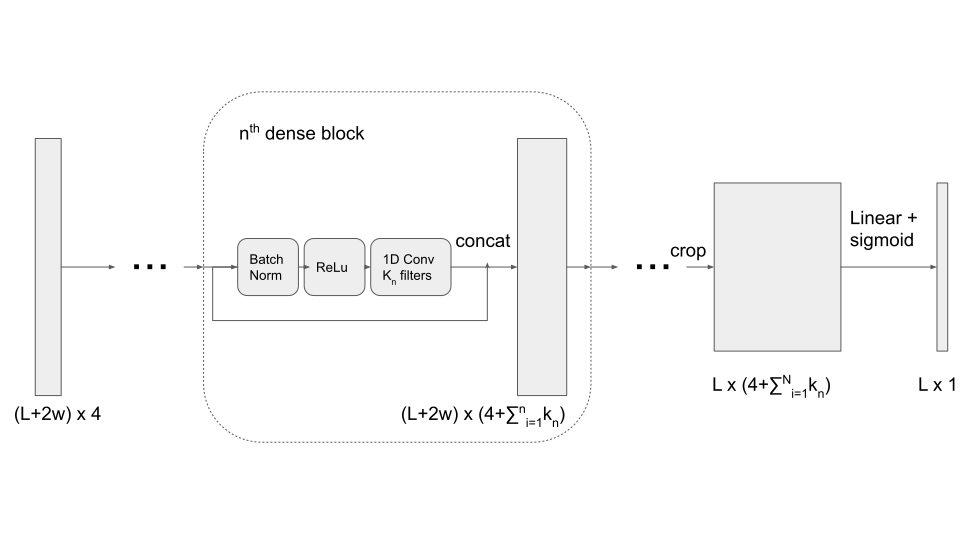
\includegraphics[width=\textwidth]{proposal_dense_net.png}
\caption{Densely connected neural network used for the yeast model}
\label{fig:dense_net}
\centering
\end{figure}

As shown in Fig\ref{fig:dense_net}, to make inference on a stretch of RNA sequence of length $L$,
we need to pad the sequence with $w$ bases on each side, where $w$ is half of the receptive field size,
as determined by all convolutional layers.
Input consists of the one-hot encoded, padded sequence,
where $A, C, G, U$ bases are encoded as $[1, 0, 0, 0], [0, 1, 0, 0], [0, 0, 1, 0], [0, 0, 0, 1]$, respectively.
The encoded input is then passed through multiple dense blocks,
where each block consists of four components:

\begin{enumerate}
    \item Batch Normalization
    \item ReLu nonlinear activation
    \item 1D dilated convolution
    \item Concatenation of the block input to the output of convolution
\end{enumerate}


\begin{table}[h!]
    \centering
    \begin{tabular}{||c c c c||}
        \hline
        Block number & Number of filters & Filter width & Dilation rate \\ [0.5ex]
        \hline\hline
        1 & 128 & 16 & 1 \\
        \hline
        2 & 128 & 16 & 2 \\
        \hline
        3 & 256 & 16 & 4 \\
        \hline
        4 & 256 & 16 & 8 \\
        \hline
        5 & 512 & 16 & 16 \\ [1ex]
        \hline
    \end{tabular}
    \caption{Dense block parameters}
    \label{table:conv_layer_params}
\end{table}

We use $5$ dense blocks in this work. The parameter of each layer is as shown in Table\ref{table:conv_layer_params}.
Densely connected block has the advantage that each block receives input from all preceding blocks,
and passes its output to all successive blocks.
The output of the last dense block essentially represents the features learnt from input at multiple resolutions.

The final dense block output is then cropped to account for the input padding,
and then passed through a fully connected layer with sigmoid activation, along the feature dimension.


\section{Training}


\begin{table}[h!]
    \centering
    \begin{tabular}{||c c||}
        \hline
        Fold number & Chromosomes \\ [0.5ex]
        \hline\hline
        1 & chrM, chrVIII, chrII, chrXV \\
        \hline
        2 & chrI, chrV, chrXIII, chrIV \\
        \hline
        3 & chrVI, chrXI, chrXVI \\
        \hline
        4 & chrIII, chrX, chrXII \\
        \hline
        5 & chrIX, chrXIV, chrVII \\ [1ex]
        \hline
    \end{tabular}
    \caption{Chromosomes used for each fold}
    \label{table:fold_chrom_split}
\end{table}


We use 5-fold cross validation, split by chromosomes, as shown in Table \ref{table:fold_chrom_split}.

Normalized data points (between $0$ and $1$) are used as soft targets without being converted to binary labels,
and models were trained using a masked cross-entropy loss, as described below.

Due to the nature of DMS modification, G/T bases has no coverage,
thus should be excluded from the calculation of the loss and the gradient.
This is achieve by first computing the per position cross-entropy loss between the prediction and the target,
then multiply it with a binary mask with the same shape as the target array.
Positions with G/T bases are being set to $0$ in the mask, while positions with A/C bases are $1$.
The masked loss are then summed over positions, and minibatch dimension,
to calculate the loss for the current minibatch and the gradient for back propagation.

Models were trained using fixed sequence length of $50$ (before padding, sequence length at inference time can be variable),
minibatch size of $10$, Adam optimizer with learning rate $0.0001$ and momentum $0.9$.
To prevent the models from overfitting, L1 and L2 regularizers with weight $0.000001$ was added to the loss,
and training is stopped if validation loss hasn't improved over the last $10$ epochs.

We trained $5$ models, each using one of the folds as validation data, and the rest as training data.


\section{Performance}


\subsection{Cross-validation performance on training dataset}

We first evaluate the model performance on training dataset.
For each transcript, we used the model that wasn't trained on its chromosome to make prediction for all A/C bases.
We computed the Spearman correlation between the prediction and the target for each transcript.
Fig \ref{fig:yeast_cv_performance} shows the distribution of Spearman correlation across all transcripts.

\begin{figure}[h!]
\includegraphics[width=\textwidth]{yeast_cv_performance.png}
\caption{Densely connected neural network used for the yeast model}
\label{fig:yeast_cv_performance}
\centering
\end{figure}

\subsection{Ribosomal RNA}

Next we used our model to predict the reactivity for all A/C bases in yeast $18S$ and $25S$ ribosomal RNAs,
both were never seen by the model (neither in the training nor validation set).

Raw read count data for $18S$ and $25S$ was downloaded from GSE45803, and was processed similarly to the training dataset,
since the experimental protocol was identical.

Correlation between prediction and the normalized read count is shown in Fig\ref{fig:yeast_r18_performance} and Fig\ref{fig:yeast_r25_performance},
where each data point is one A/C base in the corresponding transcript.
In comparison, RNAfold (window size $50$ and span $50$) achieves a correlation of $0.3217$ and $0.4529$ for $18S$ and $25S$, respectively.

\begin{figure}[h!]
\includegraphics[width=\textwidth]{yeast_r18_performance.png}
\caption{Densely connected neural network used for the yeast model}
\label{fig:yeast_r18_performance}
\centering
\end{figure}

\begin{figure}[h!]
\includegraphics[width=\textwidth]{yeast_r25_performance.png}
\caption{Densely connected neural network used for the yeast model}
\label{fig:yeast_r25_performance}
\centering
\end{figure}


\subsection{Noncoding RNAs}

To evaluate whether the model generalizes to noncoding transcripts and different experimental protocol,
we processed yeast data from the ModSeq paper\cite{talkish2014mod},
where yeast was treated with DMS or no-DMS (as control),
from which the authors identified positions that are significantly modified between treated and control,
in selected noncoding and rRNA transcripts.

For each transcript, we use our models to predict on all A/C positions,
and computed the au-ROC on how well the prediction distinguish the significantly modified bases from the rest.
We also compare the performance of our model to that of RNAfold, as shown in Fig\ref{fig:yeast_modseq_performance}.

\begin{figure}[h!]
\includegraphics[width=\textwidth]{yeast_modseq_performance.png}
\caption{Densely connected neural network used for the yeast model}
\label{fig:yeast_modseq_performance}
\centering
\end{figure}


%\section{Future Work}
%
%\begin{itemize}
%  \item Improve training and generalization performance, by making use of the raw sequencing data, and biological replicates.
%  In additional to counts of RT stops, read coverage at each position can be used to infer the confidence of calling that position paired/unpaired.
%  Transcript can be reweighted during training, according to the agreement between different biological reps.
%
%  \item Multi-resolution learning.
%\end{itemize}



%\chapter{Conclusion}
%
%one dataset that has multiple mods per sequence, so we can reconstruct colleciton of structures
%
%joint learning of accessibility and other data, e.g. chip-seq peaks


\addcontentsline{toc}{chapter}{Bibliography}
\bibliographystyle{plain}
\bibliography{proposal}

\end{document}
